% ============================================================
% Reporte: datapath-2
% Generado a partir de reportes/comun/plantilla_base.tex
% (NO edites la plantilla: cada unidad trabaja en su main.tex)
%
% Reglas de secciones y extensiones: reportes/AGENTS.md
% Compilar SIEMPRE con:
%   ../../scripts/latexbuild main.tex      (desde esta carpeta)
%   → genera build/main.pdf
% ============================================================
\documentclass[llncs]{llncs}

\usepackage[utf8]{inputenc}
\usepackage[T1]{fontenc}
\usepackage{graphicx}
\usepackage{listings}
\usepackage{hyperref}
\usepackage{xcolor}

% ---- Estilo para código VHDL (apéndice y fragmentos) ----
\lstdefinestyle{vhdl}{
  language=VHDL,
  basicstyle=\ttfamily\scriptsize,
  keywordstyle=\color{black},
  commentstyle=\color{gray}\itshape,
  stringstyle=\color{black},
  showstringspaces=false,
  breaklines=true,
  frame=single,
  rulecolor=\color{black}
}
\lstset{style=vhdl}

\begin{document}

% ============================================================
% TÍTULO Y AUTORES
% ============================================================
\title{Diseño e implementación en VHDL de un datapath
de 8 bits para sumatoria, factorial y multiplicación}

\author{Alfredo Ramírez Candia$^{1}$,%
\and Aldo Mauricio Villegas Peralta$^{1}$,%
\and Uriel Lemus Pérez$^{1}$,%
\and Santiago Silverio Flores$^{1}$,%
\and Max Ramos Martinez$^{1}$}

\authorrunning{Ramírez Candia et al.}
\institute{Equipo de Arquitectura de Computadoras,\\
Benemérita Universidad Autónoma de Puebla,\\
Puebla, México\\
\email{\{rc202375947,vp202368617,lp202362797,sf202367190,rm202376182\}@alm.buap.mx}}

\maketitle

% ============================================================
% RESUMEN  (< 100 palabras)
% ============================================================
\begin{abstract}
Resumen. Se diseñó e implementó en VHDL-2008 un datapath de 8 bits
controlado por microcódigo que calcula la sumatoria $S(n)=1+\cdots+n$, el
factorial $n!$ y el producto $A\times B$. El diseño integra ALU, acumulador,
banco de registros, multiplexores, shifter y detector de cero, más una FSM
con ROM de microinstrucciones. Se verificó con 13 testbenches autochequeados
en GHDL, obteniendo $S(5)=15$, $5!=120$ y $15\times15=225$. El flujo de
simulación con GHDL y GTKWave resultó suficiente para validar la arquitectura.
\end{abstract}

\noindent\textbf{Palabras Clave:} Arquitectura de Computadoras, Datapath,
VHDL, Microcódigo, Simulación, GHDL

% ============================================================
% 1. INTRODUCCIÓN  (1–2 cuartillas)
% ============================================================
\section{Introducción}
\label{sec:intro}

El camino de datos (\emph{datapath}) es el conjunto de registros, buses y
unidades funcionales que ejecutan las operaciones de un procesador; junto con
la unidad de control, forma el núcleo de una arquitectura de computadora.
Desde la separación entre unidad de instrucciones y unidades de ejecución del
IBM System/360 Model 91~\cite{anderson1967,anderson1967fp,flynn1967} y la
formalización de la arquitectura como la interfaz programa-máquina de
Amdahl, Blaauw y
Brooks~\cite{amdahl1964}, el diseño del datapath ha sido el problema central
de la organización de computadoras: definir qué recursos de datos existen y
cómo se encadenan para llevar a cabo un algoritmo.

La motivación de este trabajo es construir, a nivel \emph{RTL} y de forma
totalmente verificable, un datapath de 8 bits capaz de resolver tres
operaciones clásicas de la práctica de laboratorio: la sumatoria
$S(n)=1+2+\cdots+n$, el factorial $n!$ y la multiplicación $A\times B$. El
objetivo general es que la misma estructura de datos, gobernada por una
unidad de control con microcódigo, ejecute los tres algoritmos cambiando
únicamente la secuencia de microinstrucciones. Los objetivos particulares
son: (i)~modelar cada recurso como una entidad VHDL independiente, (ii)~unir
las entidades en un \emph{top} estructural y (iii)~demostrar el correcto
funcionamiento mediante testbenches autochequeados y capturas de ondas.

El artículo se organiza así. La Sección~\ref{sec:diseno} presenta el marco
teórico y la arquitectura de los módulos VHDL. La
Sección~\ref{sec:propuesta} describe la metodología experimental con
GHDL~\cite{ghdl-docs} y GTKWave~\cite{gtkwave-docs}. La
Sección~\ref{sec:simulaciones} muestra las capturas de simulación de los
módulos más importantes. La Sección~\ref{sec:resultados} analiza los
resultados obtenidos y la Sección~\ref{sec:conclusiones} cierra con las
conclusiones y el trabajo futuro. Finalmente, el
Apéndice~\ref{app:codigo} reproduce el código VHDL completo.

% ============================================================
% 2. DISEÑO TEÓRICO  (3–5 cuartillas)
% ============================================================
\section{Diseño Teórico}
\label{sec:diseno}

\subsection{Arquitectura general}

Un datapath se define por la colección de elementos de almacenamiento
(registros) y elementos combinacionales (unidades funcionales, multiplexores
y buses) que, bajo el mando de señales de control, transforman un conjunto de
datos de entrada en un resultado~\cite{amdahl1964}. En nuestro diseño el
acumulador (ACC) actúa como registro-bus principal: su salida alimenta la ALU,
el banco de registros y el buffer de salida, lo que reduce el número de
buses internos. La Figura~\ref{fig:esquema} resume el flujo de datos.

\begin{figure}[t]
  \centering
  \fbox{\parbox{0.92\textwidth}{\centering\small
  \texttt{ext1/ext2/rf\_out/sh\_out} $\rightarrow$ \textbf{mux\_sup}
  $\rightarrow$ \textbf{acumulador} (bus\_acc)\\
  \texttt{bus\_acc} $\rightarrow$ ALU.A;\quad \texttt{rf\_out} $\rightarrow$ ALU.B\\
  ALU $\rightarrow$ \textbf{mux\_inf} $\rightarrow$ \textbf{shifter}
  $\rightarrow$ \texttt{sh\_out} (realimenta mux\_sup y detector\\
  \texttt{bus\_acc} $\rightarrow$ \textbf{banco reg.} (escritura) y
  \textbf{buffer salida} $\rightarrow$ \texttt{dato\_out}}}
  \caption{Esquema del camino de datos implementado. El acumulador hace de
  bus de datos y realimenta el multiplexor superior.}
  \label{fig:esquema}
\end{figure}

El ancho de palabra es de 8 bits; toda la aritmética es módulo $2^8$, por lo
que los resultados que exceden 255 se truncan (sección de
resultados). Este ancho es suficiente para los valores de prueba ($n\le5$,
$A\times B\le225$) y mantiene la simulación didáctica.

\subsection{Módulos del datapath VHDL}

Cada recurso se implementa como una entidad VHDL-2008 independiente, siguiendo
la convención del proyecto de ``un fichero = una entidad''. Los módulos son:

\begin{itemize}
  \item \textbf{alu.vhd}. Unidad aritmético-lógica de 8 bits con tres bits de
  selección (\texttt{op\_alu}) que codifican ocho funciones: pasar $A$
  (\texttt{000}), $A+B$ (\texttt{001}), $A-B$ (\texttt{010}), $A+1$
  (\texttt{011}), $A-1$ (\texttt{100}), \texttt{OR} (\texttt{101}),
  \texttt{AND} (\texttt{110}) y \texttt{NOT} $A$ (\texttt{111}). La
  operación ``$A-1$'' se usa como contador y ``$A+B$'' como suma repetida
  para la multiplicación. La suma se implementa con el operador de
  \texttt{numeric\_std}, que en GHDL se resuelve como una cadena de acarreo
  (sumador con propagación); para reducir el retardo del acarreo se conocen
  técnicas como la suma condicional~\cite{sklansky1960}, la selección de
  acarreo~\cite{bedrij1962} o los sumadores de prefijos
  paralelos~\cite{kogge1973}, no empleadas aquí por priorizar la simplicidad
  del modelo.
  \item \textbf{acumulador.vhd}. Registro de 8 bits con \emph{write enable}
  (\texttt{wr}) y \emph{clear} (\texttt{clear}); el \emph{clear} tiene
  prioridad y el reset es asíncrono.
  \item \textbf{banco\_registros.vhd}. Banco de ocho registros de 8 bits con
  lectura combinacional de un registro (\texttt{addr}) y escritura síncrona.
  Almacena los operandos y variables de cada algoritmo ($i$, $s$, $X$, $Y$,
  $P$, etc.).
  \item \textbf{mux\_superior.vhd}. Multiplexor de 8 bits con \texttt{sel\_sup}
  de 2 bits que elige entre \texttt{ext1}, \texttt{ext2}, \texttt{rf\_out} y
  \texttt{sh\_out}. Determina la fuente que entra al acumulador.
  \item \textbf{mux\_inferior.vhd}. Multiplexor de 8 bits que elige entre la
  salida de la ALU y la salida del acumulador (\texttt{sel\_inf}).
  \item \textbf{shifter.vhd}. Desplazador lógico/aritmético de 8 bits
  (\texttt{sh}: \texttt{00} pasar, \texttt{01} izq.\ lógico, \texttt{10} der.\
  lógico, \texttt{11} der.\ aritmético).
  \item \textbf{detector\_cero.vhd}. Comparador que activa \texttt{cero}
  cuando su entrada es cero; es la condición de fin de bucle para los tres
  algoritmos.
  \item \textbf{buffer\_salida.vhd}. Buffer triestado lógico controlado por
  \texttt{out\_en} que publica el resultado final en \texttt{dato\_out}.
\end{itemize}

Todos los módulos usan \texttt{ieee.numeric\_std} y el tipo
\texttt{unsigned} para la aritmética, y \texttt{std\_logic} para las señales
de control, conforme a las definiciones del estándar
IEEE~1164~\cite{ieee1164} y del lenguaje IEEE~1076-2008~\cite{ieee1076}.

\subsection{Top estructural}

\texttt{top\_datapath.vhd} (entidad \texttt{datapath}) instancia los ocho
módulos y los interconecta con señales internas (\texttt{bus\_acc},
\texttt{rf\_out}, \texttt{alu\_out}, \texttt{mux\_inf}, \texttt{sh\_out},
\texttt{mux\_sup}). El camino crítico del diseño es
\texttt{acumulador}$\rightarrow$ALU$\rightarrow$mux inferior$\rightarrow$
shifter$\rightarrow$mux superior$\rightarrow$acumulador, que se resuelve en un
ciclo de reloj por microinstrucción. La señal \texttt{cero} se calcula sobre
la salida del shifter, es decir, sobre el valor que se escribirá en el
acumulador en el siguiente flanco, lo que permite al control decidir el salto
sin un ciclo extra.

\subsection{Unidad de control con microcódigo}

La estrategia escogida es \emph{control por microprograma}: una FSM sencilla
recorre una ROM de 128 microinstrucciones. Cada microinstrucción es un
\emph{registro} VHDL que contiene la palabra de control
(\texttt{sel\_sup}, \texttt{wr\_acc}, \texttt{clr\_acc}, \texttt{addr},
\texttt{wr\_rf}, \texttt{op\_alu}, \texttt{sel\_inf}, \texttt{sh},
\texttt{out\_en}) y el control de secuencia (\texttt{salta},
\texttt{salto\_si\_cero}, \texttt{dir}, \texttt{fin}). La dirección absoluta
se calcula como \texttt{paso} $= \mathrm{modo}\times 32 + \mathrm{micropaso}$,
de modo que cada algoritmo ocupa un bloque de 32 entradas:

\begin{itemize}
  \item \textbf{Modo 00 --- sumatoria} $S(n)$. Se carga $n$ en el registro
  $i$; luego, en un bucle, se acumula $s \leftarrow s + i$ y se decrementa
  $i$ hasta que el detector de cero marque el fin. El resultado final es
  $s$.
  \item \textbf{Modo 01 --- factorial} $n!$. Se inicializa $fact=1$ y un
  contador de veces $n-1$. El bucle externo multiplica $fact \leftarrow
  fact \cdot i$ (mediante un bucle interno de suma repetida) e incrementa
  $i$ hasta completar $n-1$ productos.
  \item \textbf{Modo 10 --- multiplicación} $A\times B$. Se cargan $A$ en
  $R3$ y $B$ en $R4$; el bucle suma $A$ a un acumulador $P$ un total de $B$
  veces mediante el contador $B$. El resultado es $P$.
\end{itemize}

El microcódigo es, literalmente, la tabla de microoperaciones del plan de
trabajo del proyecto: cada fila de la tabla se convierte en una llamada al
procedimiento \texttt{pon} que rellena una entrada de la ROM. Este enfoque
separa el \emph{qué} (algoritmo) del \emph{cómo} (recursos), principio
clásico del diseño de control microprogramado.

\subsection{Banco de registros y control de bucles}

El banco de registros de 8 posiciones evita usar registros dedicados para
cada variable y acerca el diseño a un procesador real, donde los operandos
viven en un archivo de registros direccionable. La lectura es combinacional y
la escritura síncrona, de modo que una microinstrucción puede leer un registro
y, en el mismo ciclo, escribir en el acumulador. Los bucles de los tres
algoritmos se construyen con dos recursos: el detector de cero (que aporta la
condición de terminación) y la operación $A-1$ de la ALU (que decrementa el
contador). Esta combinación de \emph{recursos compartidos} para múltiples
algoritmos es la esencia del diseño de datapaths y del paralelismo a nivel de
instrucción~\cite{tjaden1970}. El uso intensivo de operaciones \emph{sobre el
mismo bus} recuerda también al enfoque de reutilización de recursos del
360/91~\cite{anderson1967fp}.

\subsection{Verificabilidad y métodos formales}

La verificación del diseño se apoya en testbenches autochequeados, es decir,
simulación dirigida por estímulos con aserciones. La verificación por
simulación es la técnica dominante en la práctica industrial, aunque su
exhaustividad es limitada; los métodos formales (comprobación de modelos,
demostración de teoremas) aportan garantías
complementarias~\cite{gupta1992,kern1999}. Para descripciones VHDL existen
entornos como Prevail~\cite{borrione1992} y cálculos de
refinamiento~\cite{breuer1997} que permiten probar equivalencias entre
especificación e implementación. Aunque este trabajo no emplea dichos
métodos, el diseño se estructuró para ser verificable: módulos pequeños, una
única entidad por fichero y aserciones por operación. El uso de herramientas
CAD/HDL comerciales o abiertas en la enseñanza de hardware está ampliamente
documentado~\cite{puvvada1993}.

% ============================================================
% 3. PROPUESTA EXPERIMENTAL  (1 hoja)
% ============================================================
\section{Propuesta Experimental}
\label{sec:propuesta}

La metodología es de tipo cuantitativo y experimental: se describe un
conjunto de testbenches, se ejecutan sobre el modelo y se comparan los
resultados observados con los esperados analíticamente.

\subsection{Herramientas}

Se empleó GHDL~\cite{ghdl-docs} como simulador de código abierto para
VHDL-2008 (bandera \texttt{--std=08}) y GTKWave~\cite{gtkwave-docs} como
visor de ondas. Todo el flujo se ejecuta a través de los scripts oficiales del
repositorio, garantizando reproducibilidad:

\begin{itemize}
  \item \texttt{scripts/vhdl-analizar datapath-2}: analiza y compila las
  fuentes de \texttt{src/} y \texttt{tb/} con GHDL.
  \item \texttt{scripts/vhdl-sim datapath-2 tb\_<modulo>}: analiza, elabora y
  ejecuta el testbench, generando
  \texttt{vhdl/datapath-2/salidas/tb\_<modulo>.vcd}.
  \item \texttt{scripts/vhdl-wave <archivo.vcd>}: abre la captura en GTKWave
  para inspección visual.
\end{itemize}

El backend de GHDL es \emph{mcode}, es decir, solo simulación; no se realiza
síntesis, en coherencia con el objetivo del curso.

\subsection{Bancos de prueba}

Se construyeron 13 testbenches autochequeados: uno por cada módulo de
\texttt{src/} (ALU, acumulador, banco de registros, multiplexores, shifter,
detector de cero y buffer de salida), uno para el \emph{top} integrado, uno
para la unidad de control y tres de extremo a extremo, llamados
\texttt{tb\_exp1\_suma}, \texttt{tb\_exp2\_factorial} y
\texttt{tb\_exp3\_mult}. Cada testbench aplica estímulos con un reloj
peri\-ódico, comprueba las salidas con
\texttt{assert ... severity failure} y emite \texttt{report "... OK"} al
finalizar; si algún resultado fuera incorrecto, la simulación abortaría con
fallo. Por tanto, el criterio de aceptación es que \emph{ningún} testbench
produzca fallo.

\subsection{Variables y procedimiento de evaluación}

La variable independiente es el conjunto de estímulos (\texttt{modo},
operandos $n$/$A$/$B$, señales de control); la variable dependiente es
\texttt{dato\_out}. La evaluación consiste en: (1)~ejecutar cada testbench y
registrar el número de microciclos consumidos; (2)~comparar \texttt{dato\_out}
con el valor esperado; y (3)~inspeccionar las ondas de los casos
representativos. Los valores de referencia son $S(1)=1$, $S(3)=6$, $S(5)=15$,
$1!=1$, $5!=120$, $4\times3=12$, $5\times5=25$, $15\times15=225$ y
$A\times0=0$.

% ============================================================
% 4. SIMULACIONES DE VHDL  (máximo 2 hojas)
% ============================================================
\section{Simulaciones de VHDL}
\label{sec:simulaciones}

Las capturas de las Figuras~\ref{fig:alu}--\ref{fig:datapath} son
fotografías de las ventanas de GTKWave al cargar los archivos \texttt{.vcd}
que genera \texttt{scripts/vhdl-sim}. La Figura~\ref{fig:alu} muestra el
banco de pruebas de la ALU con \texttt{a=05h} y \texttt{b=03h}:
\texttt{op\_alu} recorre sus ocho códigos y \texttt{f} presenta el
resultado de cada operación. Las Figuras~\ref{fig:exp1}--\ref{fig:exp3}
presentan los tres experimentos de extremo a extremo; en todas aparecen el
reloj, el reinicio, la entrada \texttt{ext1}, el código de microinstrucción
\texttt{paso}, el contador de \texttt{ciclos}, las salidas \texttt{acc\_q} y
\texttt{dato\_out} y la bandera \texttt{fin}. Durante cada experimento
\texttt{paso} recorre los microciclos del bucle de suma repetida,
\texttt{acc\_q} acumula los parciales y, al activarse \texttt{fin},
\texttt{dato\_out} presenta el resultado.

\begin{figure}[t]
  \centering
  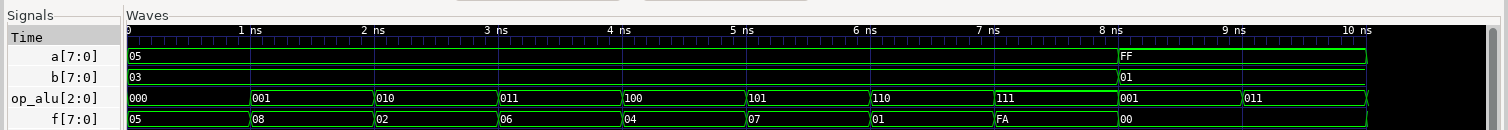
\includegraphics[width=0.72\textwidth]{figuras/captura_alu.png}
  \caption{Simulación de la ALU: las ocho operaciones de \texttt{op\_alu} y
  la salida \texttt{f} correspondiente.}
  \label{fig:alu}
\end{figure}

\begin{figure}[t]
  \centering
  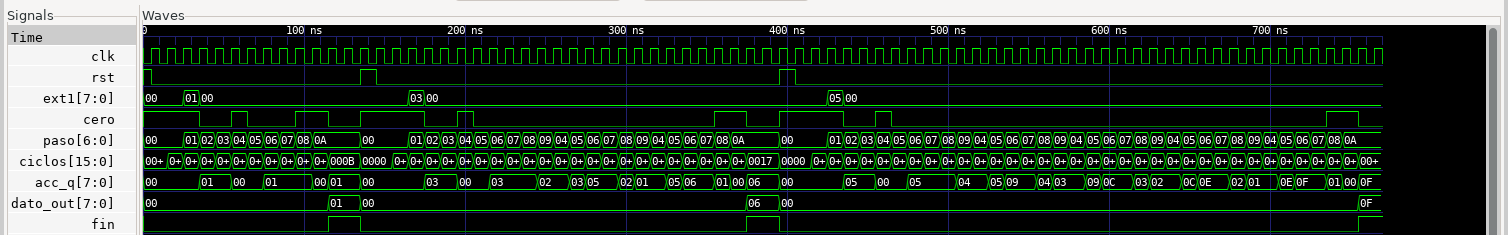
\includegraphics[width=0.98\textwidth]{figuras/captura_exp1_suma.png}
  \caption{Experimento 1 (sumatoria $S(n)$): el acumulador alcanza
  \texttt{0x0F}$=15$ y la FSM se detiene con \texttt{fin}$=1$.}
  \label{fig:exp1}
\end{figure}

\begin{figure}[t]
  \centering
  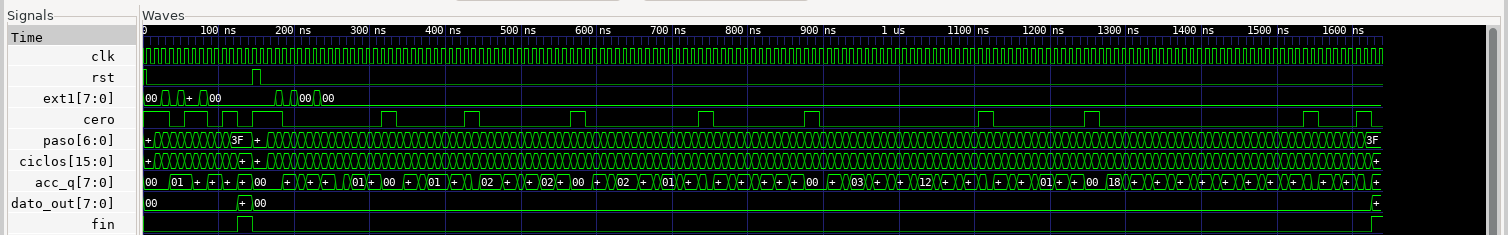
\includegraphics[width=0.98\textwidth]{figuras/captura_exp2_factorial.png}
  \caption{Experimento 2 (factorial): $5!=120$ en el acumulador; el bucle
  externo usa el bucle interno de suma repetida.}
  \label{fig:exp2}
\end{figure}

\begin{figure}[t]
  \centering
  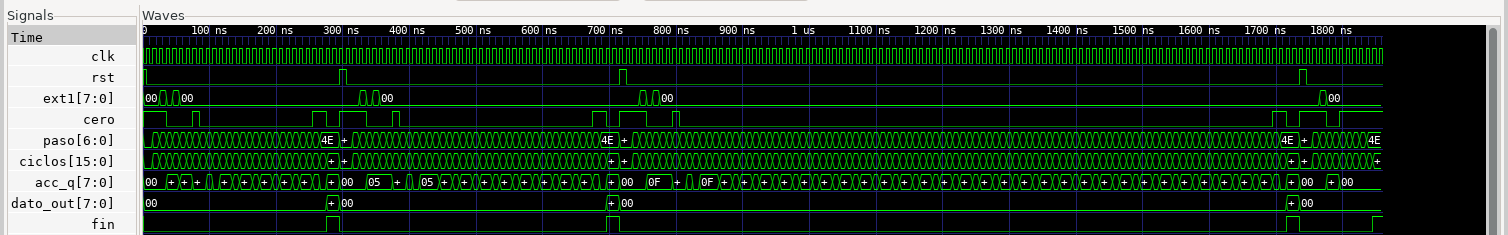
\includegraphics[width=0.98\textwidth]{figuras/captura_exp3_mult.png}
  \caption{Experimento 3 (multiplicación $A\times B$): cuatro productos
  encadenados; \texttt{dato\_out} destapa el resultado al final de cada
  bucle de suma repetida, junto al pulso de \texttt{fin}.}
  \label{fig:exp3}
\end{figure}

La Figura~\ref{fig:datapath} recoge una simulación del \emph{top} integrado
gobernada paso a paso desde el banco de pruebas, donde se aprecia la
secuencia de micro-operaciones internas (\texttt{bus\_acc},
\texttt{rf\_dout}, \texttt{cero}) junto a las señales de control
\texttt{wr\_acc}, \texttt{clr\_acc} y \texttt{wr\_rf}.

\begin{figure}[t]
  \centering
  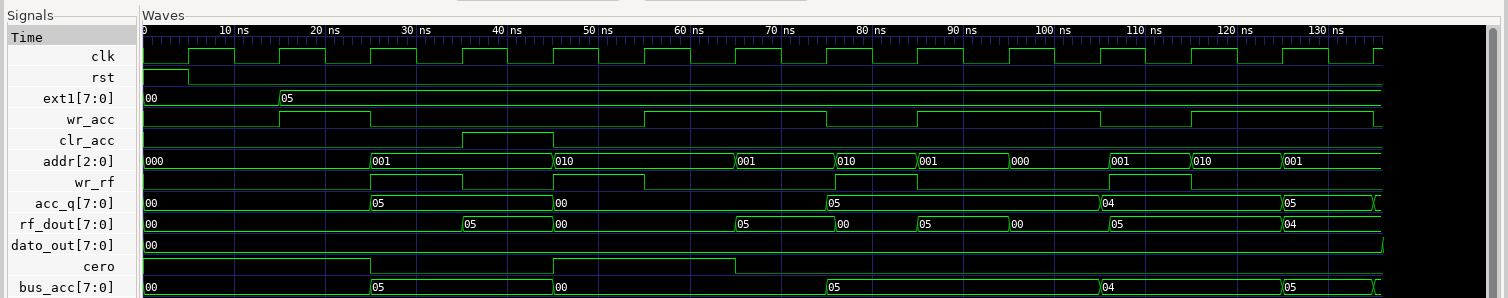
\includegraphics[width=0.98\textwidth]{figuras/captura_datapath.png}
  \caption{Simulación del datapath integrado: micro-operaciones internas y
  encadenamiento acumulador--ALU--shifter--banco.}
  \label{fig:datapath}
\end{figure}

% ============================================================
% 5. RESULTADOS  (3–5 cuartillas)
% ============================================================
\section{Resultados}
\label{sec:resultados}

\subsection{Resultados por experimento}

La Tabla~\ref{tab:resultados} resume los resultados de los tres experimentos
de extremo a extremo: valor esperado, valor simulado y número de microciclos
(\texttt{ciclos}) hasta la señal \texttt{fin}. Todos los casos coincidieron
con el valor esperado y ningún testbench emitió fallo.

\begin{table}[t]
  \caption{Resultados de los experimentos de extremo a extremo
  (aritmética de 8 bits, módulo 256).}
  \label{tab:resultados}
  \centering
  \small
  \begin{tabular}{llcc}
    \hline
    \textbf{Experimento} & \textbf{Entrada} & \textbf{Esperado} & \textbf{Microciclos}\\
    \hline
    Sumatoria $S(n)$   & $n=1$ & 1   & ---\\
    Sumatoria $S(n)$   & $n=3$ & 6   & ---\\
    Sumatoria $S(n)$   & $n=5$ & 15  & ---\\
    Factorial $n!$     & $n=1$ & 1   & ---\\
    Factorial $n!$     & $n=5$ & 120 & 147\\
    Multiplicación     & $4\times3$   & 12  & ---\\
    Multiplicación     & $5\times5$   & 25  & ---\\
    Multiplicación     & $15\times15$ & 225 & ---\\
    Multiplicación     & $A\times0$   & 0   & ---\\
    \hline
  \end{tabular}
\end{table}

Los valores de $n$ bajos ($n=1$, $3$) y de productos pequeños se eligieron
para verificar la correcta inicialización y los caminos de un solo paso; los
valores mayores ejercitan los bucles internos y externos. El caso $A\times0$
verifica que el detector de cero termina el bucle antes de ejecutar ninguna
suma, devolviendo 0.

\subsection{Verificación de los módulos base}

Los 13 testbenches (10 de módulos y control, 3 de extremo a extremo)
finalizaron con 13 \texttt{OK} y 0 \texttt{FAIL}. Este resultado tiene dos
lecturas. Por un lado, valida cada recurso de forma aislada: por ejemplo, la
ALU produce correctamente las ocho funciones y el shifter aplica los cuatro
modos de desplazamiento. Por otro, la prueba de integración confirma que el
encadenamiento estructural y las señales de control son coherentes. La
verificación por simulación es la técnica estándar en el flujo de diseño
digital y, aunque no es exhaustiva, combinada con aserciones por operación
ofrece una confianza razonable para un diseño didáctico~\cite{kern1999}.

\subsection{Análisis del consumo de microciclos}

El caso $5!$ consumió 147 microciclos, coherente con su estructura de dos
bucles anidados: el bucle externo recorre $i=2..5$ (cuatro productos) y cada
producto ejecuta un bucle interno de suma repetida. La multiplicación
$A\times B$ consume microciclos proporcionales a $B$, pues el bucle interno
suma $A$ exactamente $B$ veces. La sumatoria $S(n)$, en cambio, consume
microciclos proporcionales a $n$ (un ciclo de acumulación y decremento por
iteración). Esta diferencia ilustra un compromiso de diseño clásico: la
\emph{misma} ALU sirve para los tres algoritmos, pero el costo temporal depende
del algoritmo. Un multiplicador dedicado reduciría el producto a una sola
operación; sin embargo, el objetivo aquí era maximizar la reutilización de
recursos con una ALU simple, enfoque que recuerda a las unidades de ejecución
que comparten un único camino de
datos~\cite{anderson1967fp,tjaden1970}.

\subsection{Observación de las ondas}

En las capturas se distinguen tres fases en cada experimento: una de
\emph{inicialización} (microciclos que cargan constantes y operandos en el
banco), una de \emph{cómputo} (los bucles) y una de \emph{salida} (la
microinstrucción final activa \texttt{out\_en} y \texttt{fin}). La señal
\texttt{paso} avanza de uno en uno en el bloque correspondiente al
\texttt{modo} elegido, y los saltos se manifiestan como discontinuidades en
\texttt{paso}, justo cuando el detector de cero activa la condición
\texttt{salto\_si\_cero}. La visibilidad de estas transiciones valida la
unidad de control microprogramada.

\subsection{Limitaciones}

La principal limitación es el ancho fijo de 8 bits y la aritmética módulo
$2^8$: $n!$ desborda para $n\ge6$ ($6!=720>255$) y el producto desborda para
$A\times B>255$. El diseño no implementa banderas de \emph{overflow} ni
extensión de signo, de modo que los resultados desbordados se truncan
silenciosamente. Además, la comparación se limitó a simulación (backend
\emph{mcode}): no se realizó síntesis ni estimación de área o frecuencia. Estas
limitaciones son aceptables para el alcance didáctico del trabajo, pero
deberían abordarse si el datapath se integrara en un diseño mayor.

% ============================================================
% 6. CONCLUSIONES  (1 cuartilla)
% ============================================================
\section{Conclusiones}
\label{sec:conclusiones}

Se diseñó, implementó y verificó en VHDL-2008 un datapath de 8 bits capaz de
ejecutar tres algoritmos (sumatoria, factorial y multiplicación) mediante una
unidad de control microprogramada. El diseño cumple los objetivos planteados:
cada recurso es una entidad independiente, el \emph{top} estructural los
integra y los 13 testbenches autochequeados pasan sin fallo, con resultados
correctos ($S(5)=15$, $5!=120$, $15\times15=225$). La reutilización de la ALU
y el banco de registros para los tres algoritmos demuestra el principio de
diseño de recursos compartidos que caracteriza a los datapaths reales.

Como trabajo futuro se propone: (i)~ampliar el ancho de palabra o añadir
detección de desbordamiento; (ii)~extender el microcódigo con nuevas
operaciones, aprovechando que la ROM reserva bloques de 32 entradas por modo;
(iii)~explorar un multiplicador dedicado frente a la suma repetida; y
(iv)~incorporar métodos de verificación formal~\cite{gupta1992,borrione1992}
para complementar la simulación.

% ============================================================
% REFERENCIAS  (>= 15)
% ============================================================
\bibliographystyle{splncs04}
\bibliography{referencias}

% ============================================================
% APÉNDICE — CÓDIGO VHDL
% ============================================================
\appendix
\section{Código VHDL}
\label{app:codigo}

Se reproduce a continuación el código completo de los módulos de
\texttt{vhdl/datapath-2/src/}. Las capturas de ondas y el flujo de
simulación se describen en las Secciones~\ref{sec:simulaciones}
y~\ref{sec:resultados}.

\subsection{ALU}
\lstinputlisting[caption={alu.vhd --- unidad aritmético-lógica de 8 bits},
label=lst:alu]{../../vhdl/datapath-2/src/alu.vhd}

\subsection{Acumulador}
\lstinputlisting[caption={acumulador.vhd --- registro-bus con clear},
label=lst:acc]{../../vhdl/datapath-2/src/acumulador.vhd}

\subsection{Banco de registros}
\lstinputlisting[caption={banco\_registros.vhd --- 8 registros de 8 bits},
label=lst:rf]{../../vhdl/datapath-2/src/banco_registros.vhd}

\subsection{Multiplexores}
\lstinputlisting[caption={mux\_superior.vhd --- selección de fuente al acumulador},
label=lst:muxsup]{../../vhdl/datapath-2/src/mux_superior.vhd}
\lstinputlisting[caption={mux\_inferior.vhd --- ALU o acumulador},
label=lst:muxinf]{../../vhdl/datapath-2/src/mux_inferior.vhd}

\subsection{Shifter y detector de cero}
\lstinputlisting[caption={shifter.vhd --- desplazamiento lógico/aritmético},
label=lst:sh]{../../vhdl/datapath-2/src/shifter.vhd}
\lstinputlisting[caption={detector\_cero.vhd --- comparación con cero},
label=lst:cero]{../../vhdl/datapath-2/src/detector_cero.vhd}

\subsection{Buffer de salida}
\lstinputlisting[caption={buffer\_salida.vhd --- buffer triestado de salida},
label=lst:out]{../../vhdl/datapath-2/src/buffer_salida.vhd}

\subsection{Top estructural}
\lstinputlisting[caption={top\_datapath.vhd --- integración de los módulos},
label=lst:top]{../../vhdl/datapath-2/src/top_datapath.vhd}

\subsection{Unidad de control}
\lstinputlisting[caption={control.vhd --- FSM y ROM de microinstrucciones},
label=lst:ctrl]{../../vhdl/datapath-2/src/control.vhd}

\end{document}
